\chapter{Distributed Hash Tables}
\begin{figure}[htbp]
   \centering
   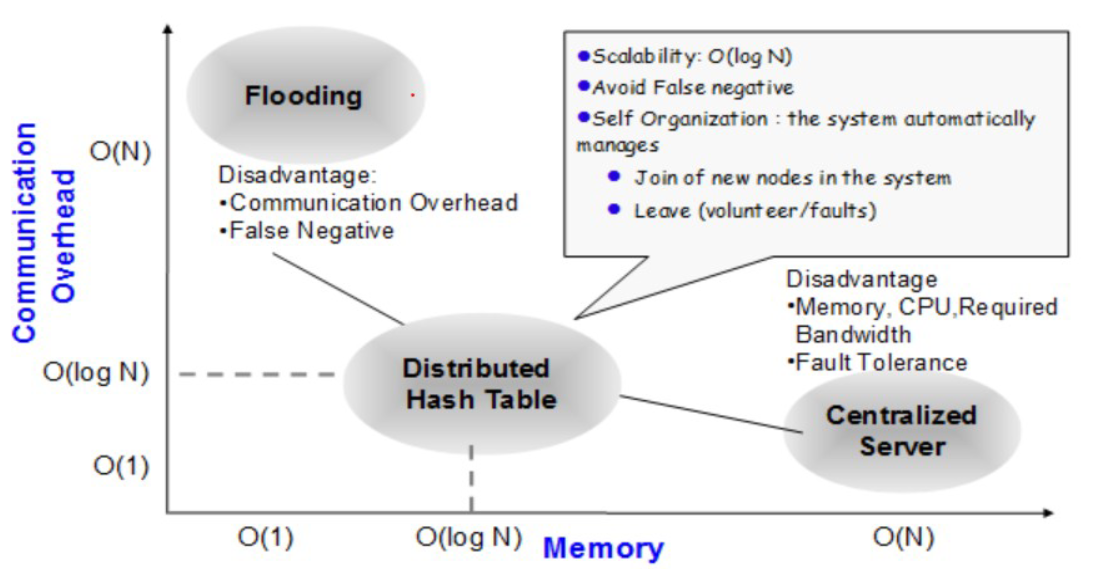
\includegraphics{images/DHT_motivations.png}
   \caption{DHT Motivations}
   \label{fig:DHT_motivations}
\end{figure}

The key idea is to split the hash tables into several parts and distribute them to several servers, and to use hash of resources (or of the URLs of resources) as a key to map them to a
dynamically changing set of web caches, but with \ul{each key mapped to single server}; so that
each machine (user) can locally compute which web cache should contain the
required resource, refenced by an URL.\\
This technique is extended to DHT for P2P systems.

However, \ul{\textbf{rehashing} is a problem in dynamic scenarios} if the hashing scheme depends directly on the number of servers:
$99\%$ of keys have to be remapped, resulting in a lot of messages exchange.
\begin{figure}[htbp]
   \centering
   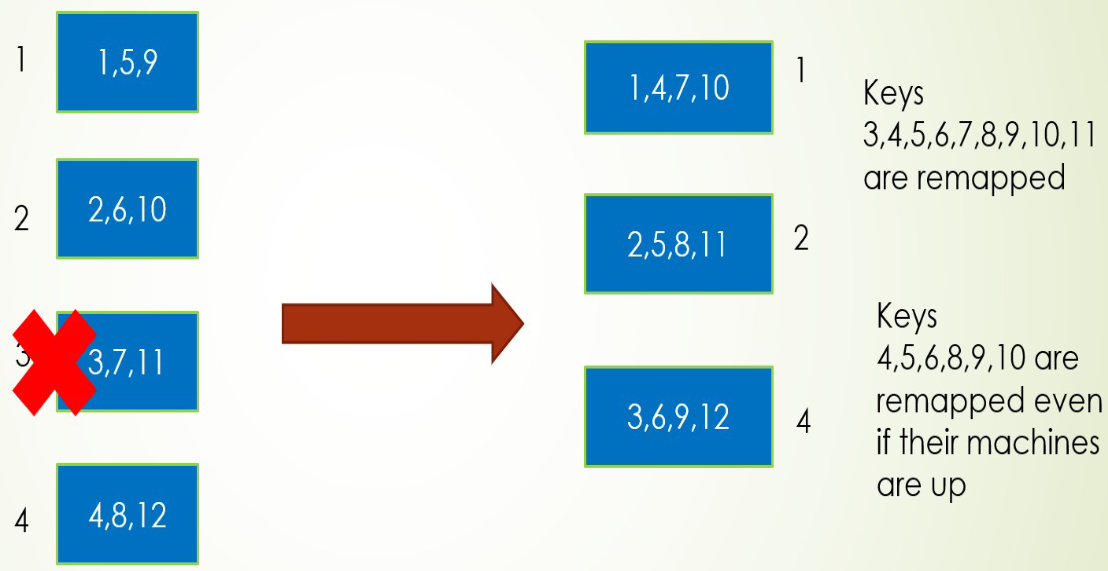
\includegraphics{images/rehashing_problem.png}
   \caption{Rehashing problem}
   \label{fig:rehashing_problem}
\end{figure}

\textbf{Consistent hashing} is a set of hash techniques which guarantees that adding more nodes/remove nodes implies \ul{moving only a minority of data items}.
each node manages ---instead of a set of sparse keys--- an interval of consecutive hash keys, and intervals are joined/splitted when nodes join/leave the network and keys redistributed between adjacent peers.


\section{Building CHORD DHT}
\begin{paracol}{2}
   % \colfill
   \begin{itemize}
      \item Use a logical name space, called \textit{identifier space} consisting of identifiers
      $\{0,1,2,...,N-1\}$
      \item define identifier space as a \textit{logical ring} modulo $N$
      \item every node picks a random identifier
      through Hash function $H$.
      \item the function \texttt{succ(x)} returns the node with an identifier $\geq x$.
      \item every item $v$ to be stored gets assigned to \texttt{succ(H(v))}
   \end{itemize}
   \begin{figure}[htbp]
      \centering
      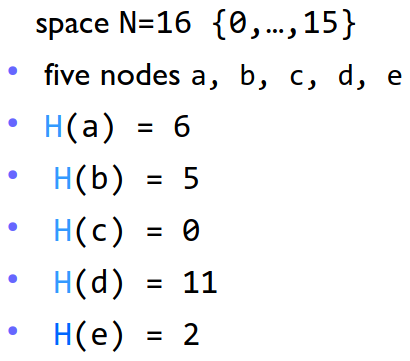
\includegraphics{images/DHT_build2.png}
      % \caption{}
      \label{fig:DHT_build2}
   \end{figure}

   % \colfill
   \switchcolumn
   
   % \begin{adjustbox}{valign=\fill}
   \begin{figure}[htbp]
      \centering
      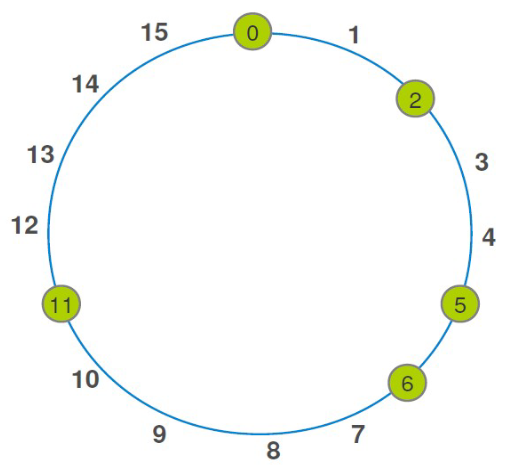
\includegraphics{images/DHT_build1.png}
      \caption{Identifier space}
      In this figure, the node identifiers are 16 and the green circles indicate which are the online nodes.
      \label{fig:DHT_build1}
   \end{figure}
   % \end{adjustbox}
   
\end{paracol}

\subsection{Peers joining and leaving}
When a new node is \textbf{added}, we map the keys between the new node and the previous node in the hash ring to point to the new node;\\
those the keys will no longer be associated with their old nodes.

When a node is \textbf{removed} from the hash ring, only the keys associated with that node are rehashed and remapped rather than remapping all the keys.

In case a node suddenly disconnects from the network, all data stored on it are lost if they are not stored on other nodes;
to avoid such a problem:
\begin{itemize}
   \item introduce some redundancy (data replication)
   \item information loss: periodical information refresh
\end{itemize}

\begin{figure}[htbp]
   \centering
   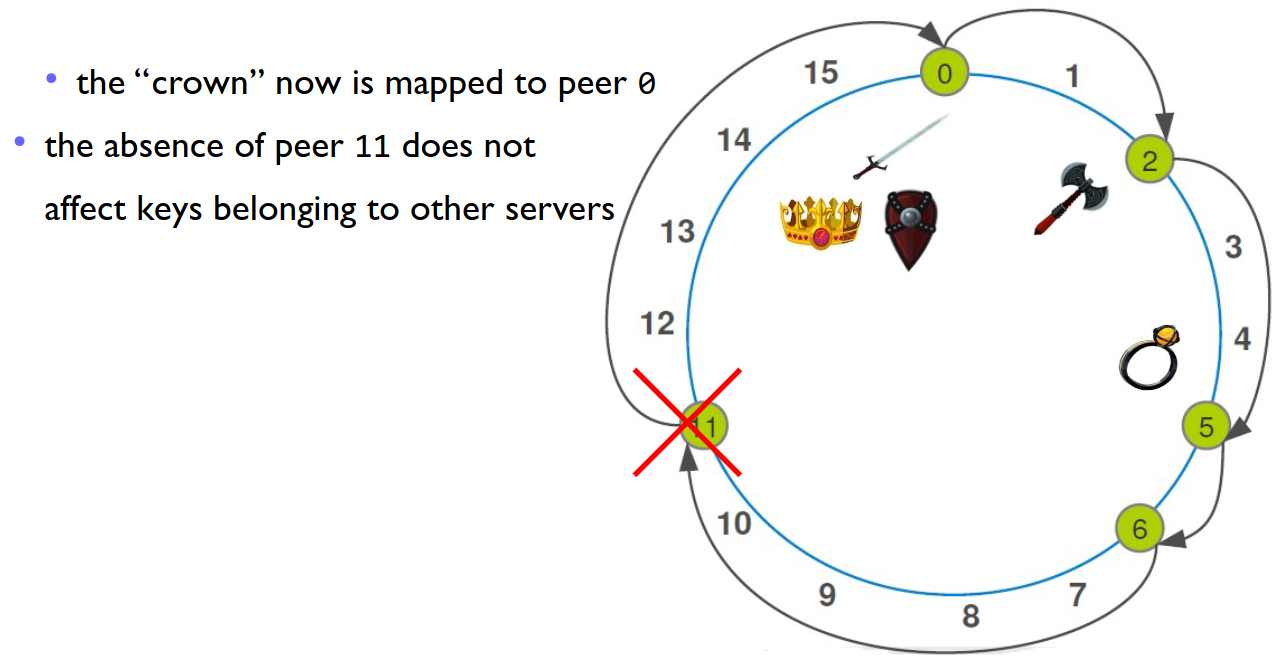
\includegraphics{images/p2p_peerleaves.png}
   \caption{Peer 11 leaves the Network}
   \label{fig:p2p_peerleaves}
   In case a peer leaves, its keys can easily be remapped to its successor
\end{figure}

When the hash table is \textbf{resized}, on the average,only $\frac{k}{n}$ keys need to be remapped on average, where $k$ is the number of keys and $n$ is the number of servers.
\newpage
\section{Finger Table and Data Lookup}

\begin{figure}[htbp]
   \centering
   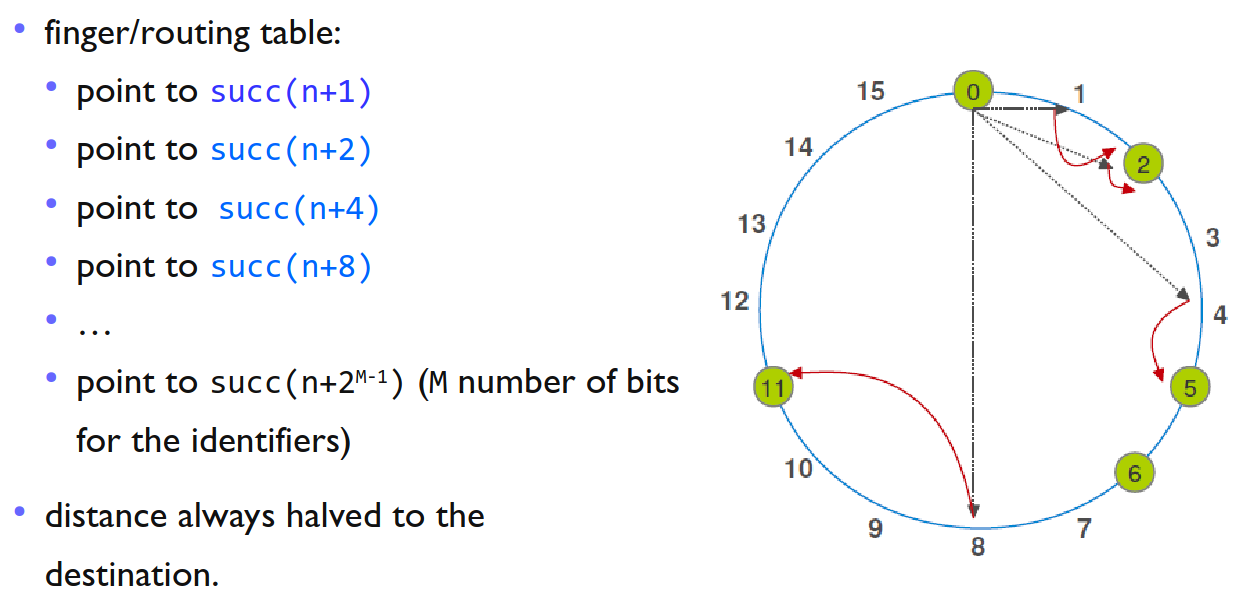
\includegraphics{images/dht_exponentialsearch.png}
   \caption{Finger table for CHORD DHT}
   The data lookup can be implemented by using exponential search, rather than performing a walk by asking each peer for its successor
   \label{fig:dht_exponentialsearch}
\end{figure}

\begin{figure}[htbp]
   \centering
   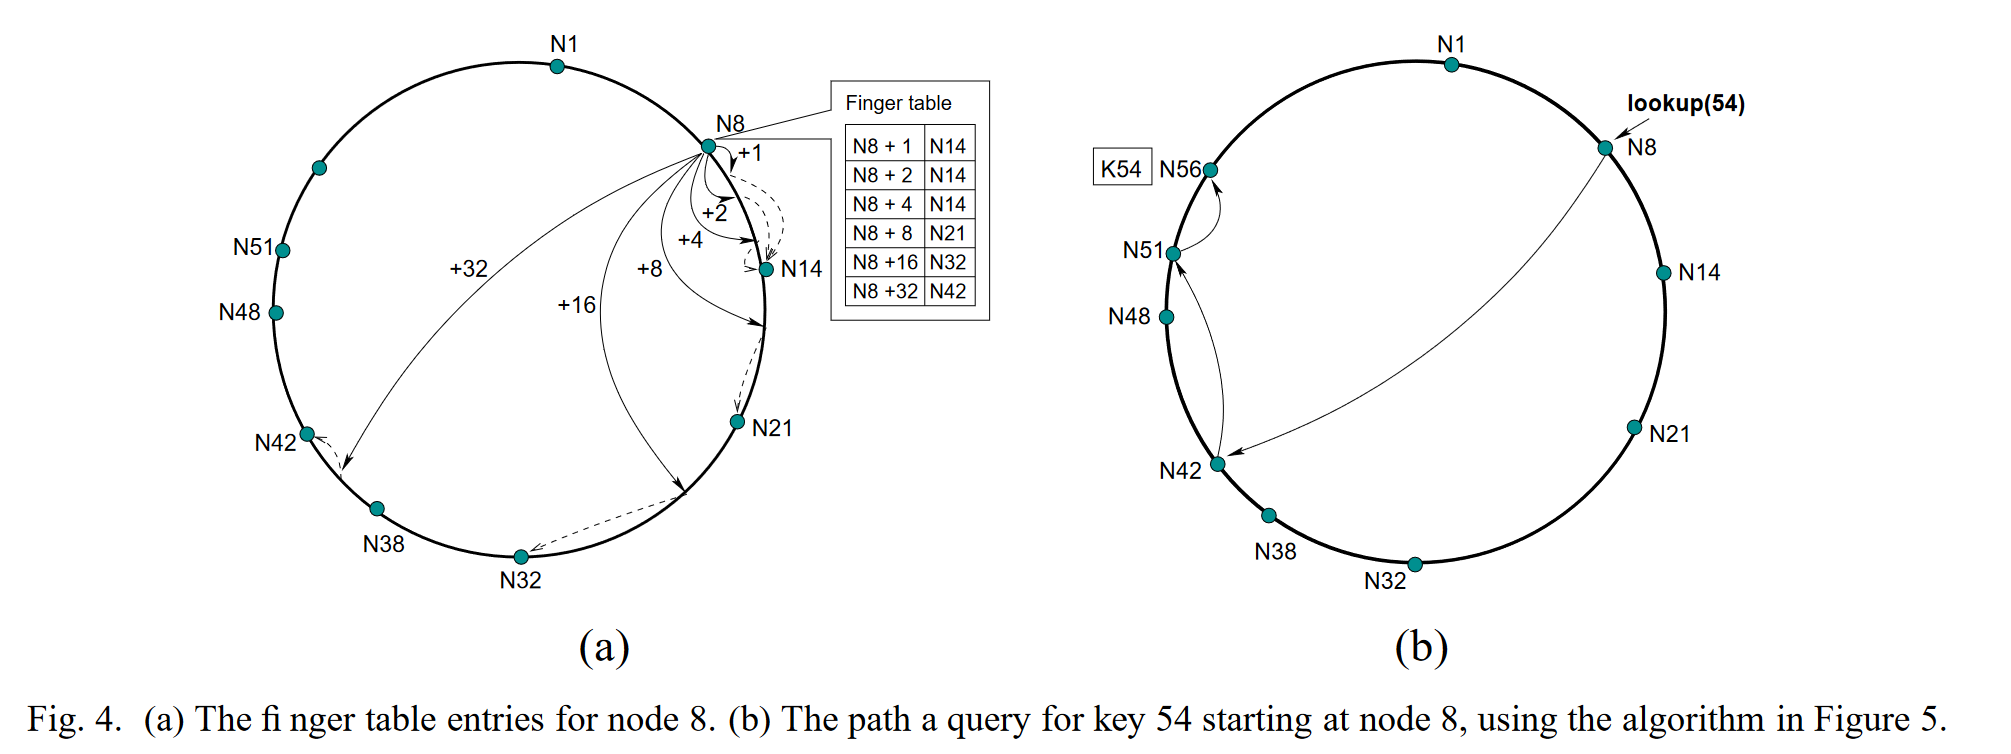
\includegraphics{images/dht_chordfinger.png}
   \caption{This image is a bit more precise than the previous one}
   \label{fig:dht_chordfinger}
   Each $k^{th}$ \textbf{finger} for the node $n$ is defined as $finger[k] = succ(n+2^{k-1})$, i.e. the first node on the circle that succeeds $n+2^{k-1} mod 2^m$, having $1 \leq k \leq m$. 
\end{figure}

\begin{paracol}{2}
   \colfill
   The lookup algorithm, instead of walking through successors to find the desired key, can be sped up by using the \textbf{finger table}.
   Here is the algorithm, which is logarithmic in the number of nodes.
   The use of finger tables not only allows to speed up the search, but also to reduce the number of nodes each peer has to keep track of.

   \note{In Fig. \ref{fig:dht_chordfinger} node 8 the successor of 54 he knows of is 1, which does not contain the key 54, so then 8 finds the closest preceding node to 54 in its finger table, which is 42, which finds again as successor of 54 the node 1, since he knows only $succ(42+8)=51$ and $succ(42+16)=1$, so asks 51 (closest preceding node) to find the successor of 54, which is 56 (finally \smiley).}
   \colfill
   \switchcolumn
   \begin{lstlisting}[mathescape=true,basicstyle={\footnotesize\ttfamily},language=Haskell]
// ask node n to find the successor of id
n.find successor(id)
   if (id $\in$ (n, successor])
      return successor;
   else
      n' = closest preceding node(id );
      return n'.find successor(id);
// search the local table for the highest predecessor of id
n.closest preceding node(id)
   for i = m downto 1
      if (finger[i] $\in$ (n, id))
         return finger[i];
   return n;  
   \end{lstlisting}
\end{paracol}

So, \textbf{Data Lookup} is performed by computing the hash $h(x)$ of the searched object, asking for $succ(h(x))$ whether they have $x$, and if not, propagating the query to farthest node\footnote{Which is found using the finger table} which has an identifier smaller than $h(x)$, which then recursively applies the same algorithm, until the object $x$ is found.
\begin{figure}[htbp]
   \centering
   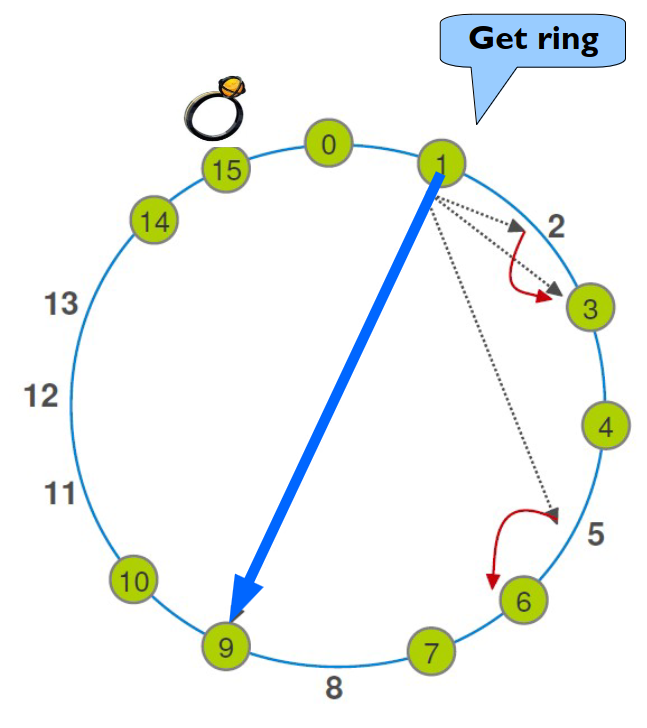
\includegraphics[width=0.3\columnwidth]{images/dht_chordsearch01.png}
   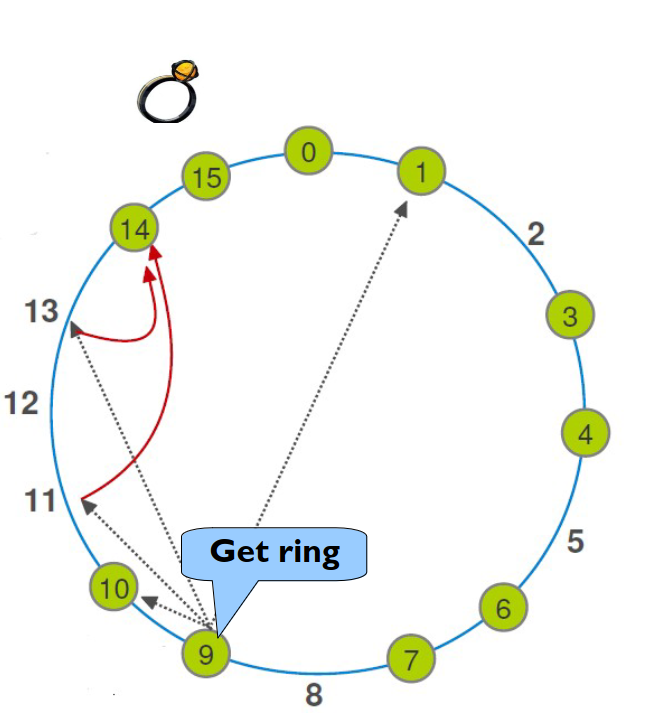
\includegraphics[width=0.3\columnwidth]{images/dht_chordsearch02.png}\\
   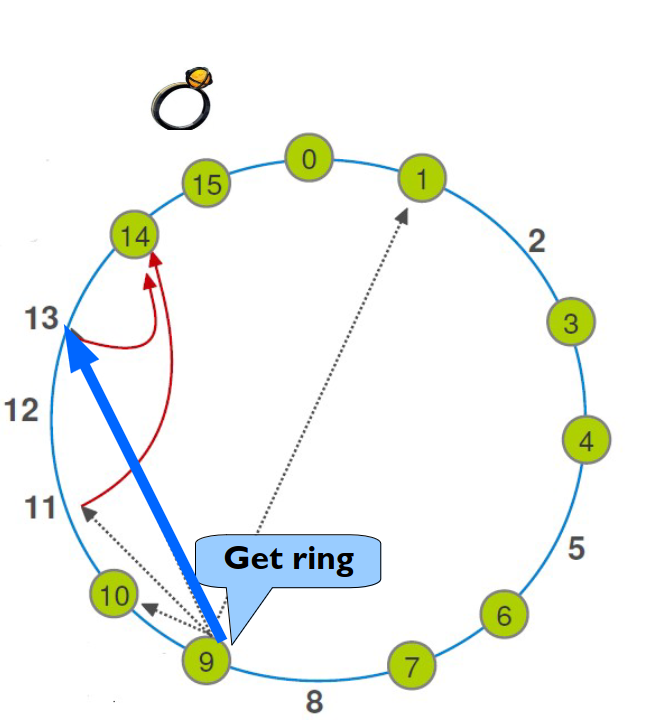
\includegraphics[width=0.3\columnwidth]{images/dht_chordsearch03.png}
   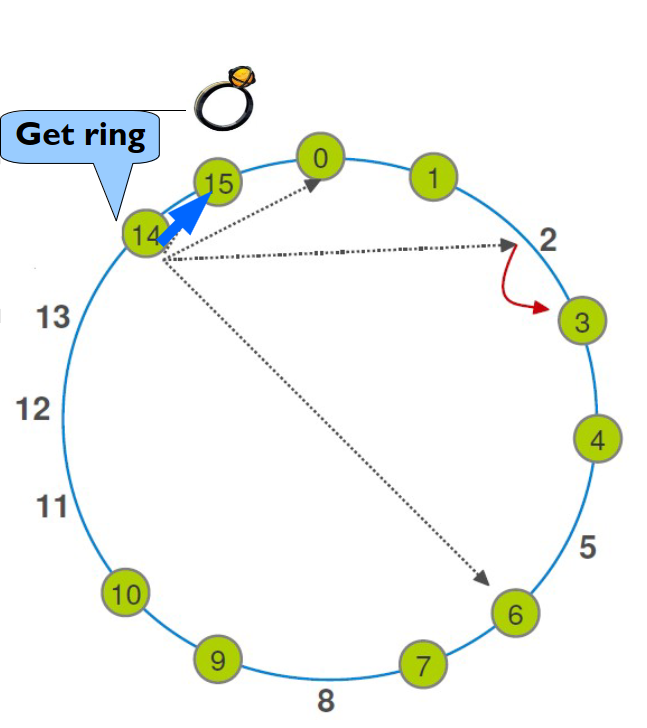
\includegraphics[width=0.3\columnwidth]{images/dht_chordsearch04.png}
   \caption{Lookup performed in the \texttt{\textbf{CHORD}} DHT}
   Dotted arrows here indicate the nodes each peer knows of, and the big solid arrows indicate the path the query follows to find the desired key.
   \label{fig:dht_chordsearch}
\end{figure}

\subsection{Addressing data}
Data was usually addressed by \textbf{location}, a \texttt{http://} link to locate resources;
Such link is an identifier that points to a particular location on the web.\\
This approach forces us all to \ul{pretend that the data are in only one location}.

IPFS instead uses \textbf{content addressing}, which exploits the cryptographic hash of the content to identify it.

\subsection{API, Lookup and Various Properties}
To avoid having a node managing a bigger portion of the identifier space, a uniform hash function may be used.\\
Most DHT provide a simple inferface \texttt{PUT,GET,Value}, usually \textit{without} the possibility to move keys.

\begin{figure}[htbp]
   \centering
   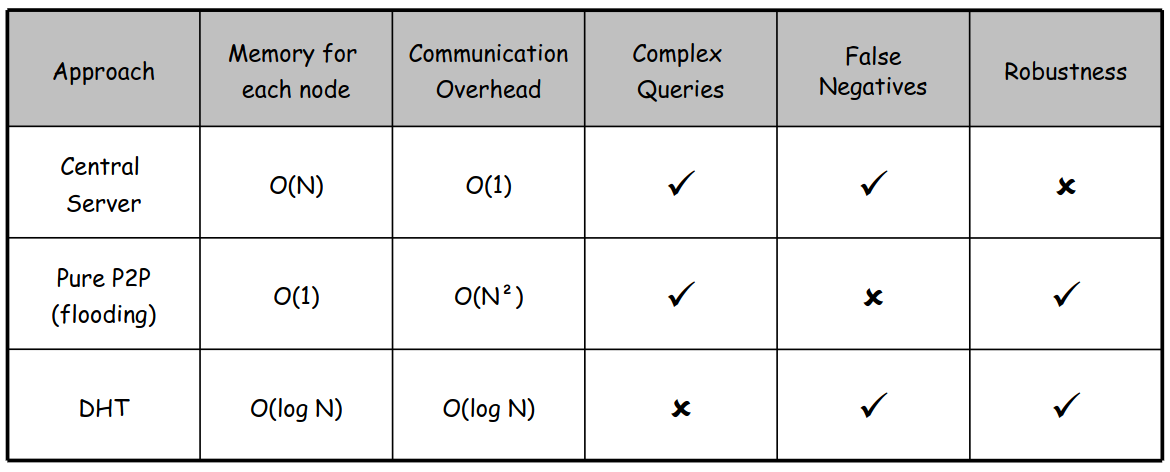
\includegraphics{images/DHT_lookupcomplexity.png}
   \caption{Lookup time complexity comparison}
   \label{fig:DHT_lookupcomplexity}
\end{figure}

\labelitemize{\textit{DHT}}{
   \begin{itemize}
      \item Routing is based on key (unique identifier)
      \item Key are uniformly distributed to the DHT nodes
      \begin{enumerate}
         \item Bottleneck avoidance
         \item Incremental insertion of the keys
         \item Fault tolerance
      \end{enumerate}
      \item Auto organizing system
      \item Simplex and efficient organization
      \item The terms “Structured Peer-to-Peer“ and “DHT“ are often used as
      synonyms
   \end{itemize}
}